\chapter{Entwicklung des Prototpys für Visual Studio Code}
\label{cha:EntwicklungVsCode}

\section{Design}
\label{sec:EntwicklungVsCode_Design}

\begin{figure}
    \centering
    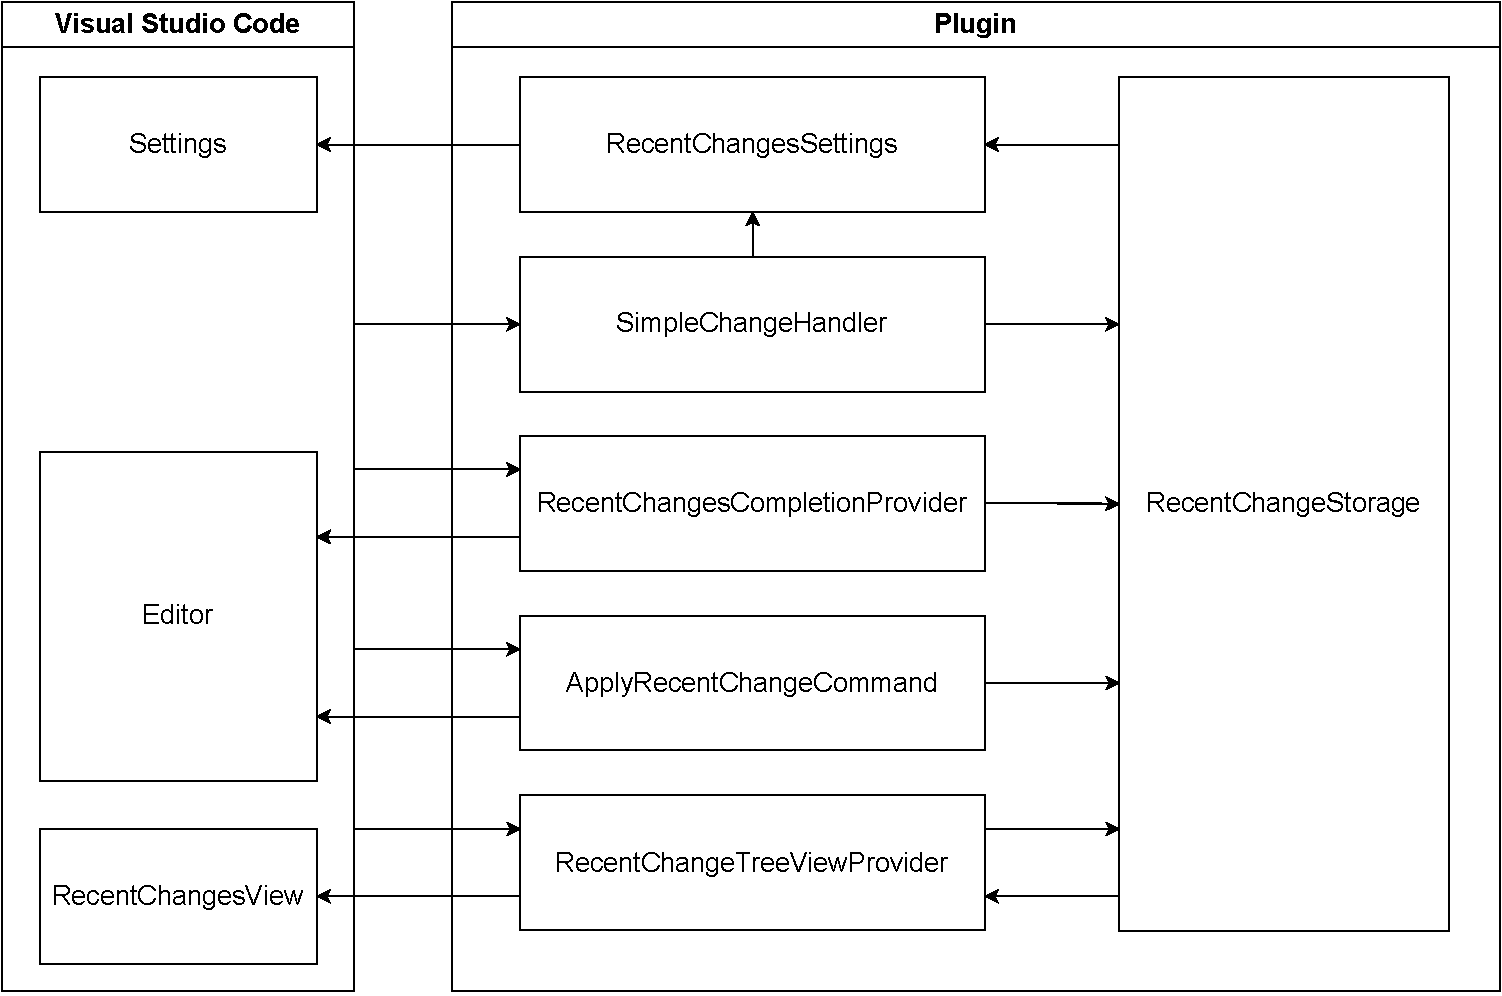
\includegraphics[width=.95\textwidth]{diagram_VSCodeDesign-Simplified}
    \caption{Stark vereinfachte Übersicht über das Design des Plugins in  VS Code.}
    \label{fig:diagram_VSCodeDesign-Simplified}
\end{figure}   
\begin{figure}
    \centering
    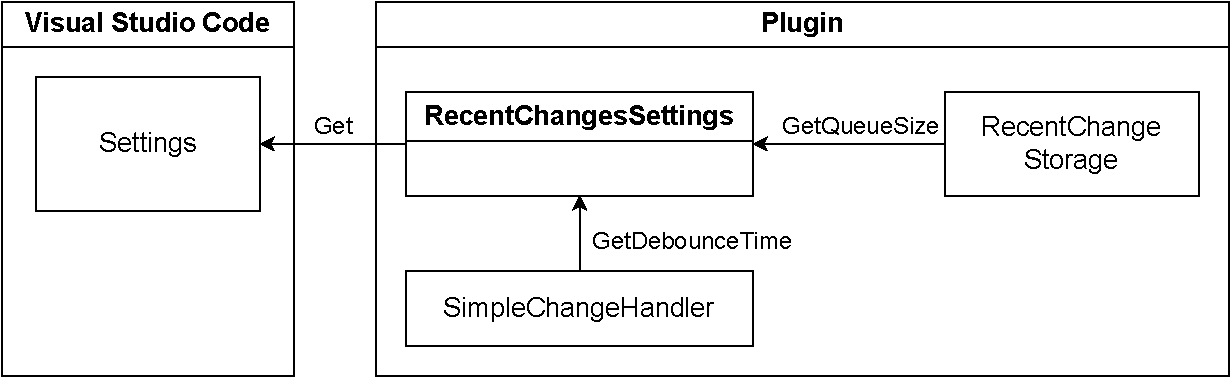
\includegraphics[width=.95\textwidth]{diagram_VSCodeDesign-Detail_Settings}
    \caption{Detaillierte Darstellung der Komponente \emph{RecentChangesSettings}.}
    \label{fig:diagram_VSCodeDesign-Detail_Settings}
\end{figure}   
\begin{figure}
    \centering
    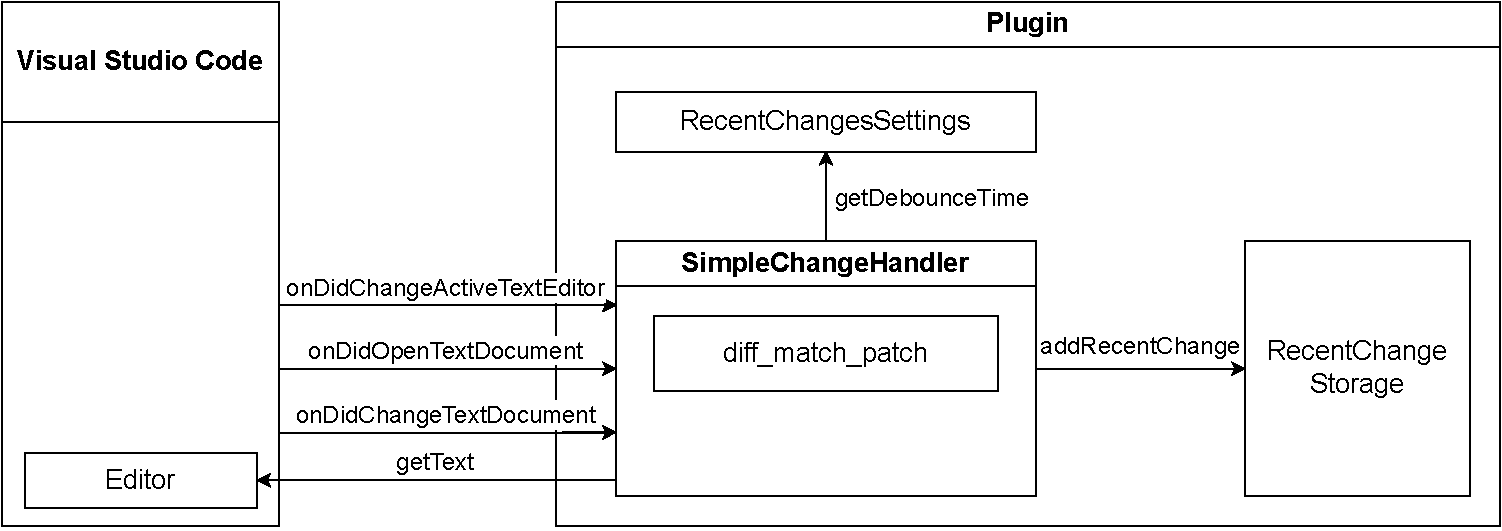
\includegraphics[width=.95\textwidth]{diagram_VSCodeDesign-Detail_Handler}
    \caption{Detaillierte Darstellung des \emph{SimpleChangeHandler}.}
    \label{fig:diagram_VSCodeDesign-Detail_Handler}
\end{figure}   
\begin{figure}
    \centering
    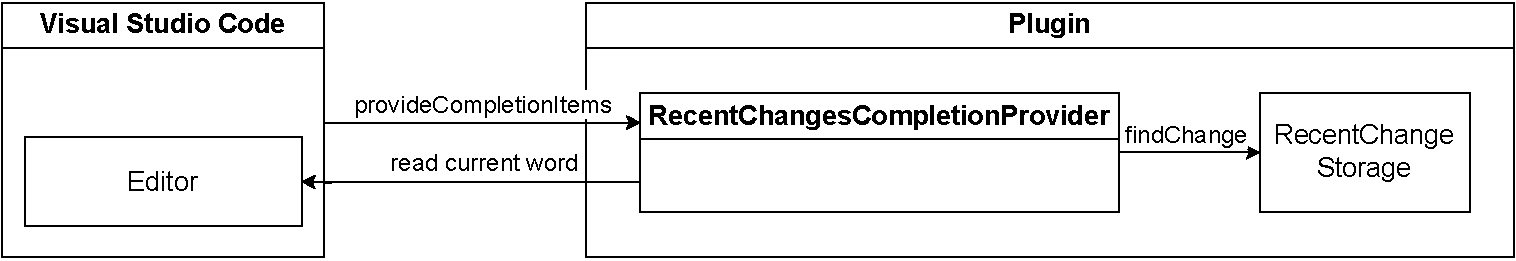
\includegraphics[width=.95\textwidth]{diagram_VSCodeDesign-Detail_Provider}
    \caption{Detaillierte Darstellung des \emph{RecentChangesCompletionProvider}.}
    \label{fig:diagram_VSCodeDesign-Detail_Provider}
\end{figure}   
\begin{figure}
    \centering
    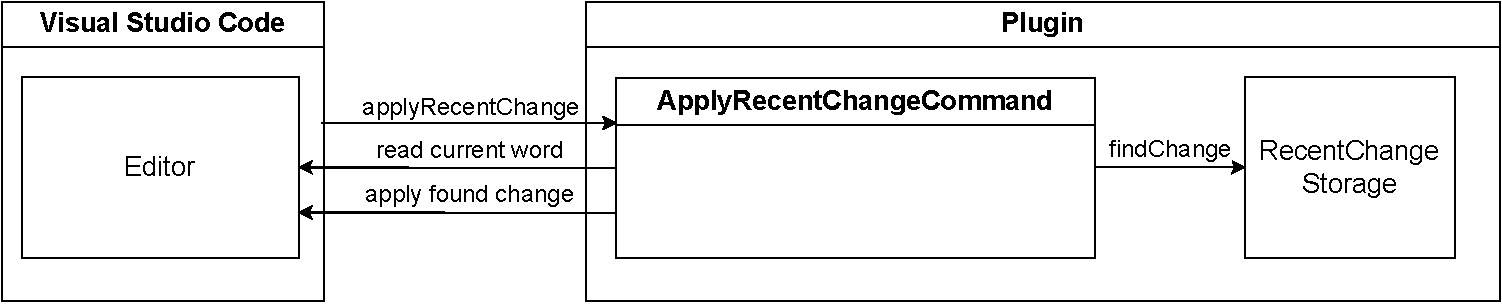
\includegraphics[width=.95\textwidth]{diagram_VSCodeDesign-Detail_Command}
    \caption{Detaillierte Darstellung des \emph{ApplyRecentChangeCommand}.}
    \label{fig:diagram_VSCodeDesign-Detail_Command}
\end{figure}   
\begin{figure}
    \centering
    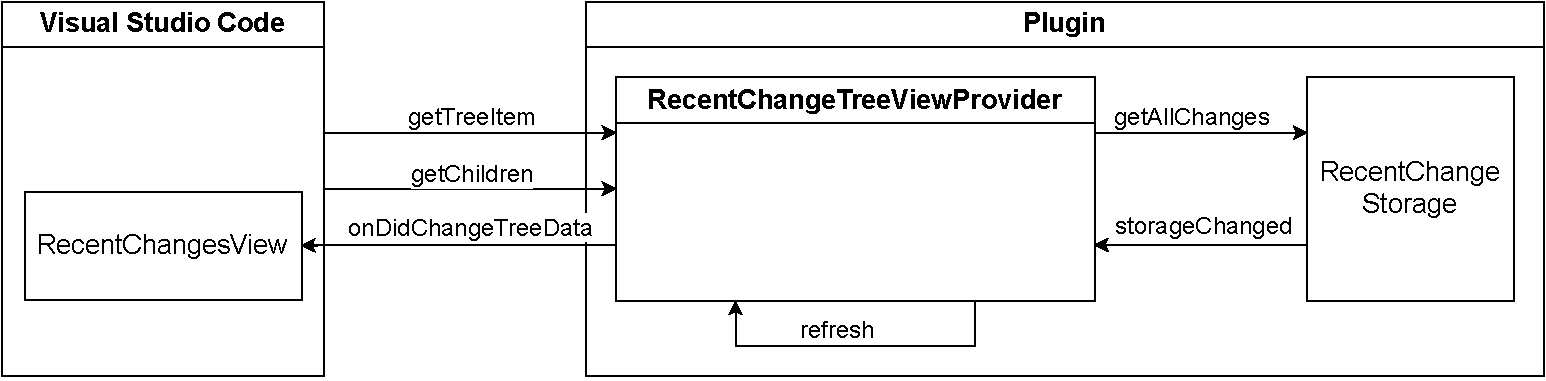
\includegraphics[width=.95\textwidth]{diagram_VSCodeDesign-Detail_TreeView}
    \caption{Detaillierte Darstellung des \emph{RecentChangeTreeViewProvider}.}
    \label{fig:diagram_VSCodeDesign-Detail_TreeView}
\end{figure}   
\begin{figure}
    \centering
    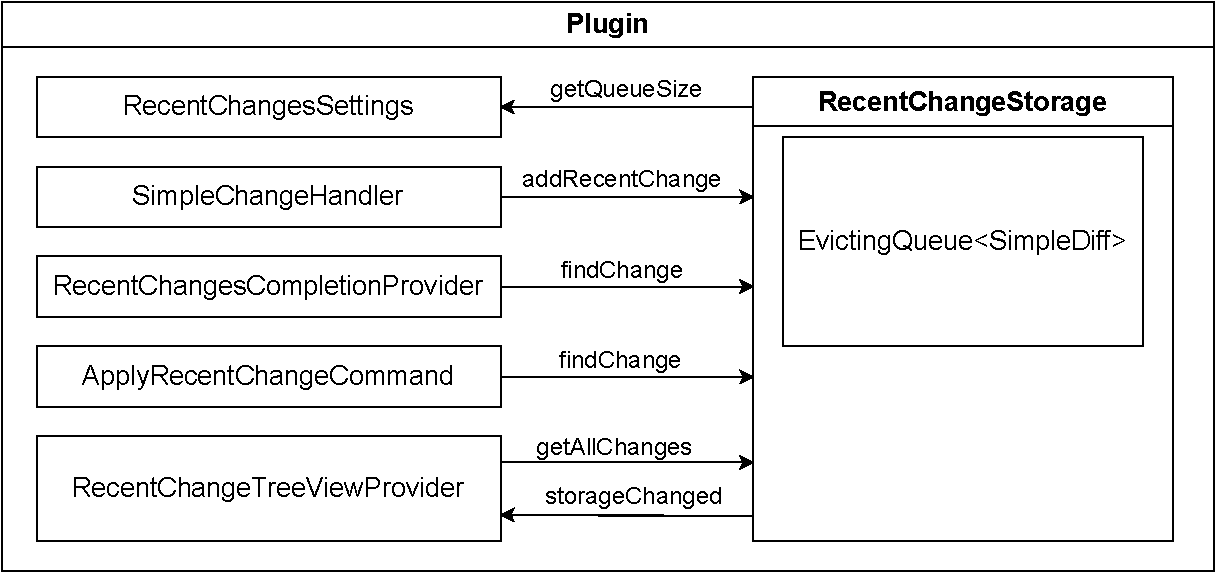
\includegraphics[width=.95\textwidth]{diagram_VSCodeDesign-Detail_Storage}
    \caption{Detaillierte Darstellung des \emph{RecentChangeStorage}.}
    \label{fig:diagram_VSCodeDesign-Detail_Storage}
\end{figure}   

\section{Implementierung}
\label{sec:EntwicklungVsCode_Implementierung}

\subsection{Aufsetzen des Projektes}

\subsubsection{Aufbau der Ordnerstruktur}

\subsection{Entwicklung}

\section{Tests}
\label{sec:EntwicklungVsCode_Tests}

\section{Publishing}
\label{sec:EntwicklungVsCode_Publishing}

\section{CI/CD}
\label{sec:EntwicklungVsCode_CICD}